
%
%We demonstrate these contributions by changing the input to our molecular
%dynamics simulation, which changes the keyspace access patterns. 
%
%\subsection{Structured Access Regimes}
%
%Figures~\ref{fig:keyspace-analysis_size},~\ref{fig:keyspace-analysis_locality} and~\ref{fig:keyspace-analysis_throughput}.
%%shows ``access regimes", or groups of accesses
%%to the same subset of keys:
%\begin{itemize}
%  \item change immediately, different sizes
%  \item monotonically increasing
%  \item random access to a single key
%  \item early keys accessed more
%\end{itemize}
%
%\noindent\textbf{Conclusion}: unique patterns of a real HPC application
%
%\subsection{Cache Size Analysis}
%
%Figure~\ref{fig:keyspace-analysis_cachesize}.
%
%\noindent\textbf{Conclusion}: workload phases (high request rate to a small
%number of keys and then low request rate to a large number keys) need a dynamic
%load balancing policy.
%
%\subsection{Overfitting Policies}
%
%Figures~\ref{fig:keyspace-analysis_cachesize-dynamic} and~\ref{fig:keyspace-analysis_cachesize-caveats}.
%
%\noindent\textbf{Side Idea}: we need to figure out what ParSplice memory is
%sensitive to: max usage or usage over time.\\
%
%\noindent\textbf{Conclusion}: dynamic policies absorb the cost of a high read
%request rate for a 2.5 hour run, but it is infeasible to do this for every
%combination of system setup, job lengths, parsplice parameters.
%
%\subsubsection*{Discussion}
%Why don't we just an LRU cache:
%\begin{itemize}
%  \item we can do better (workload is structured and has locality)
%  \item finding the size of the cache is hard
%  \item hotspots dissipate too quickly
%\end{itemize}

\section{ParSplice Keyspace Analysis}
\label{sec:parsplice-keyspace-analysis}

\begin{figure}[t]
\noindent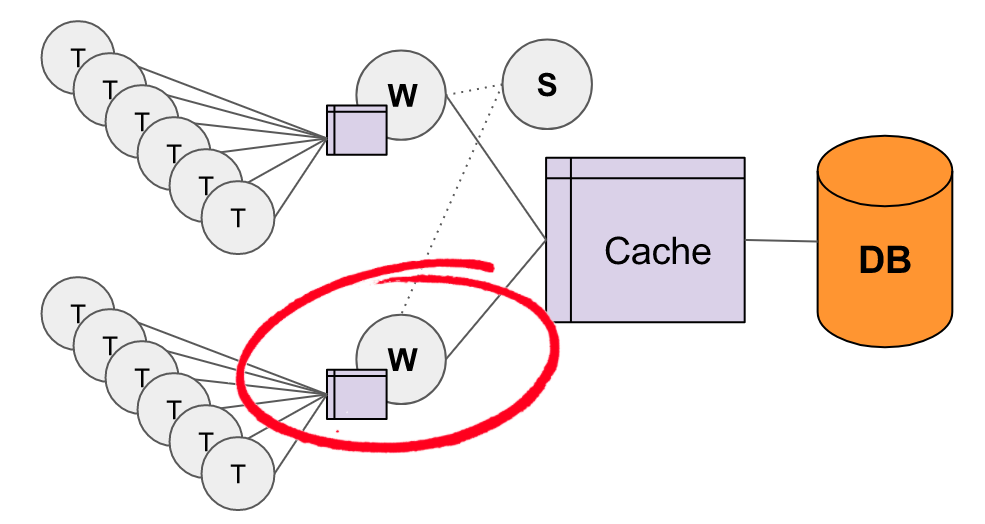
\includegraphics[width=0.5\textwidth]{figures/parsplice.png}\\
\caption{The ParSplice architecture has a storage hierarchy of caches and a
dedicated cache node (boxes) backed by a persistent database (DB). A splicer
(S) tells worker (W) to generate segments and workers employ tasks (T) for more
parallelization. We focus on the worker's cache (circled), which facilitates
communication and segment exchange between the worker and its
\label{fig:parsplice}}
\end{figure}

ParSplice~\cite{perez:jctc20150parsplice} is an accelerated molecular dynamics
(MD) simulation package developed at LANL. It is part of the Exascale Computing
Project\footnote{http://www.exascale.org/bdec/} and is important to LANL's
Materials for the Future initiative. As shown in Figure~\ref{fig:parsplice},
the phases are:

\begin{enumerate}

  \item a splicer tells workers to generate segments (short MD trajectory) for
  specific states

  \item workers read initial coordinates for their assigned segment from data
  store; the key-value pair is (state ID, coordinate)

  \item upon completion, workers insert final coordinates for each segment into
  data store, and wait for new segment assignment

\end{enumerate}

The computation can be parallelized by adding more workers or by adding tasks
to parallelize individual workers.  The workers are stateless and read initial
coordinates from the data store each time they begin generating segments. Since
worker tasks do not maintain their own history, they can end up reading the
same coordinates repeatedly. To mitigate the consequences of these repeated
reads, ParSplice provisions a hierarchy of processes to act as caches that sit
in front of a single persistent database.  Values are written to each tier and
reads traverse up the hierarchy until they find the data.  Caches also reside
on the workers to service reads/writes from its tasks.  

We use ParSplice to simulate the evolution of metallic nanoparticles that grow
from the vapor phase.  This simulation stresses the storage hierarchy more than
other input decks because it uses a cheap potential, has a small number of
atoms, and operates in a complex energy landscape with many accessible states.
As the run progresses, the energy landscape of the system becomes more complex
and more states are visited.  Two domain factors control the number of entries
in the data store: the growth rate and the temperature. The growth rate
controls how quickly new atoms are added to the nanoparticle: fast growth rates
lead to non-equilibrium conditions, and hence increase the number of states
that can be visited.  However, as the particle grows, the simulation slows down
because the calculations become more expensive, limiting the rate at which new
states are visited.  On the other hand, the temperature controls how easily a
trajectory can jump from state to state; higher temperatures lead to more
frequent transitions but temperatures that are too high result in meaningless
simulations because trajectories have so much energy that they are equally
likely to visit any random state. 

Changing growth rates and temperature alters the size, shape, and locality of
the data store keyspace. Lower temperatures and smaller growth rates create
hotter keys with smaller keyspaces as many segments are generated in the same
set of states before the trajectory can escape to a new region of state space.
In Figure~\ref{fig:motivation-regimes}, the \(\Delta_1\) growth rate adds atoms
every 100K microseconds while the \(\Delta_2\) growth rate adds atoms every 1
million microseconds. So \(\Delta_2\) has a smaller growth rate resulting in
hotter keys (line on \(y1\) axis) and a smaller keyspace (dots on the \(y2\)
axis).  Values smaller than \(\Delta_2\)'s growth rate or a temperature of 400
degrees results in very little database activity because state transitions take
too long. Similarly, values larger than \(\Delta_1\)'s growth rate or a
temperature of 4000 degrees result in an equally meaningless simulation as
transitions are unrealistic.

Our evaluation uses the total ``trajectory length" as the goodness metric. This
value is the duration of the overall trajectory produced by ParSplice. At
ideal efficiency, the trajectory length should increase with the square root of
the wall-clock time, since the wall-clock cost of time-stepping the system by
one simulation time unit increases in proportion of the total number of atoms.

\subsection{ParSplice Keyspace Analysis}
\label{sec:parsplice-keyspace-analysis}
%IT HAS 8K keys!  How did we take these measurements

We instrumented ParSplice with performance counters and keyspace counters.  The
performance counters track ParSplice progress while keyspace counters track
which keys are being accessed by the ParSplice ranks. Because the keyspace
counters have high overhead we only turn them on for the keyspace analysis.

\subsubsection*{Experimental Setup} All experiments ran on Trinitite, a Cray
XC40 with 32 Intel Haswell 2.3GHz cores per node.  Each node has 128GB of RAM
and our goal is to limit the size of the cache to 3\% of
RAM\footnote{Empirically, we find this threshold works well for most
applications}. Note that this is an addition to the 30GB that ParSplice uses to
manage other ranks on the same node.  A single Cray node produced trajectories
that are \(5\times\) times longer than our 10 node CloudLab clusters and
\(25\times\) longer than our 10 node cluster at UCSC. As a result, it reaches
different job phases faster and gives us a more comprehensive view of the
workload. The performance gains compared to the commodity clusters have more to
do with memory/PCI bandwidth than network.

The scalability experiment uses 1 splicer, 1 persistent database, 1 cache
process, and up to 2 workers. We scale up to 1024 tasks, which spans 32 nodes
and disable hyper-threading because we experience unacceptable variability in
performance. For the rest of the experiments, we use 4 nodes, 1 splicer, 1
persistent database, 1 cache process, 1 worker, and up to 512 tasks.  The
keyspace analysis that follows is for the cache on the worker node, which is
circled in Figure~\ref{fig:parsplice}.  The cache hierarchy is unmodified but
for the persistent database node, we replace BerkeleyDB on NFS with LevelDB on
Lustre. Original ParSplice experiments showed that BerkeleyDB's syncs caused
reads/writes to bottleneck on the persistent database. We also use Riak's
customized LevelDB\footnote{https://github.com/basho/leveldb} version, which
comes instrumented with its own set of performance counters.

\begin{figure}[t]
  \noindent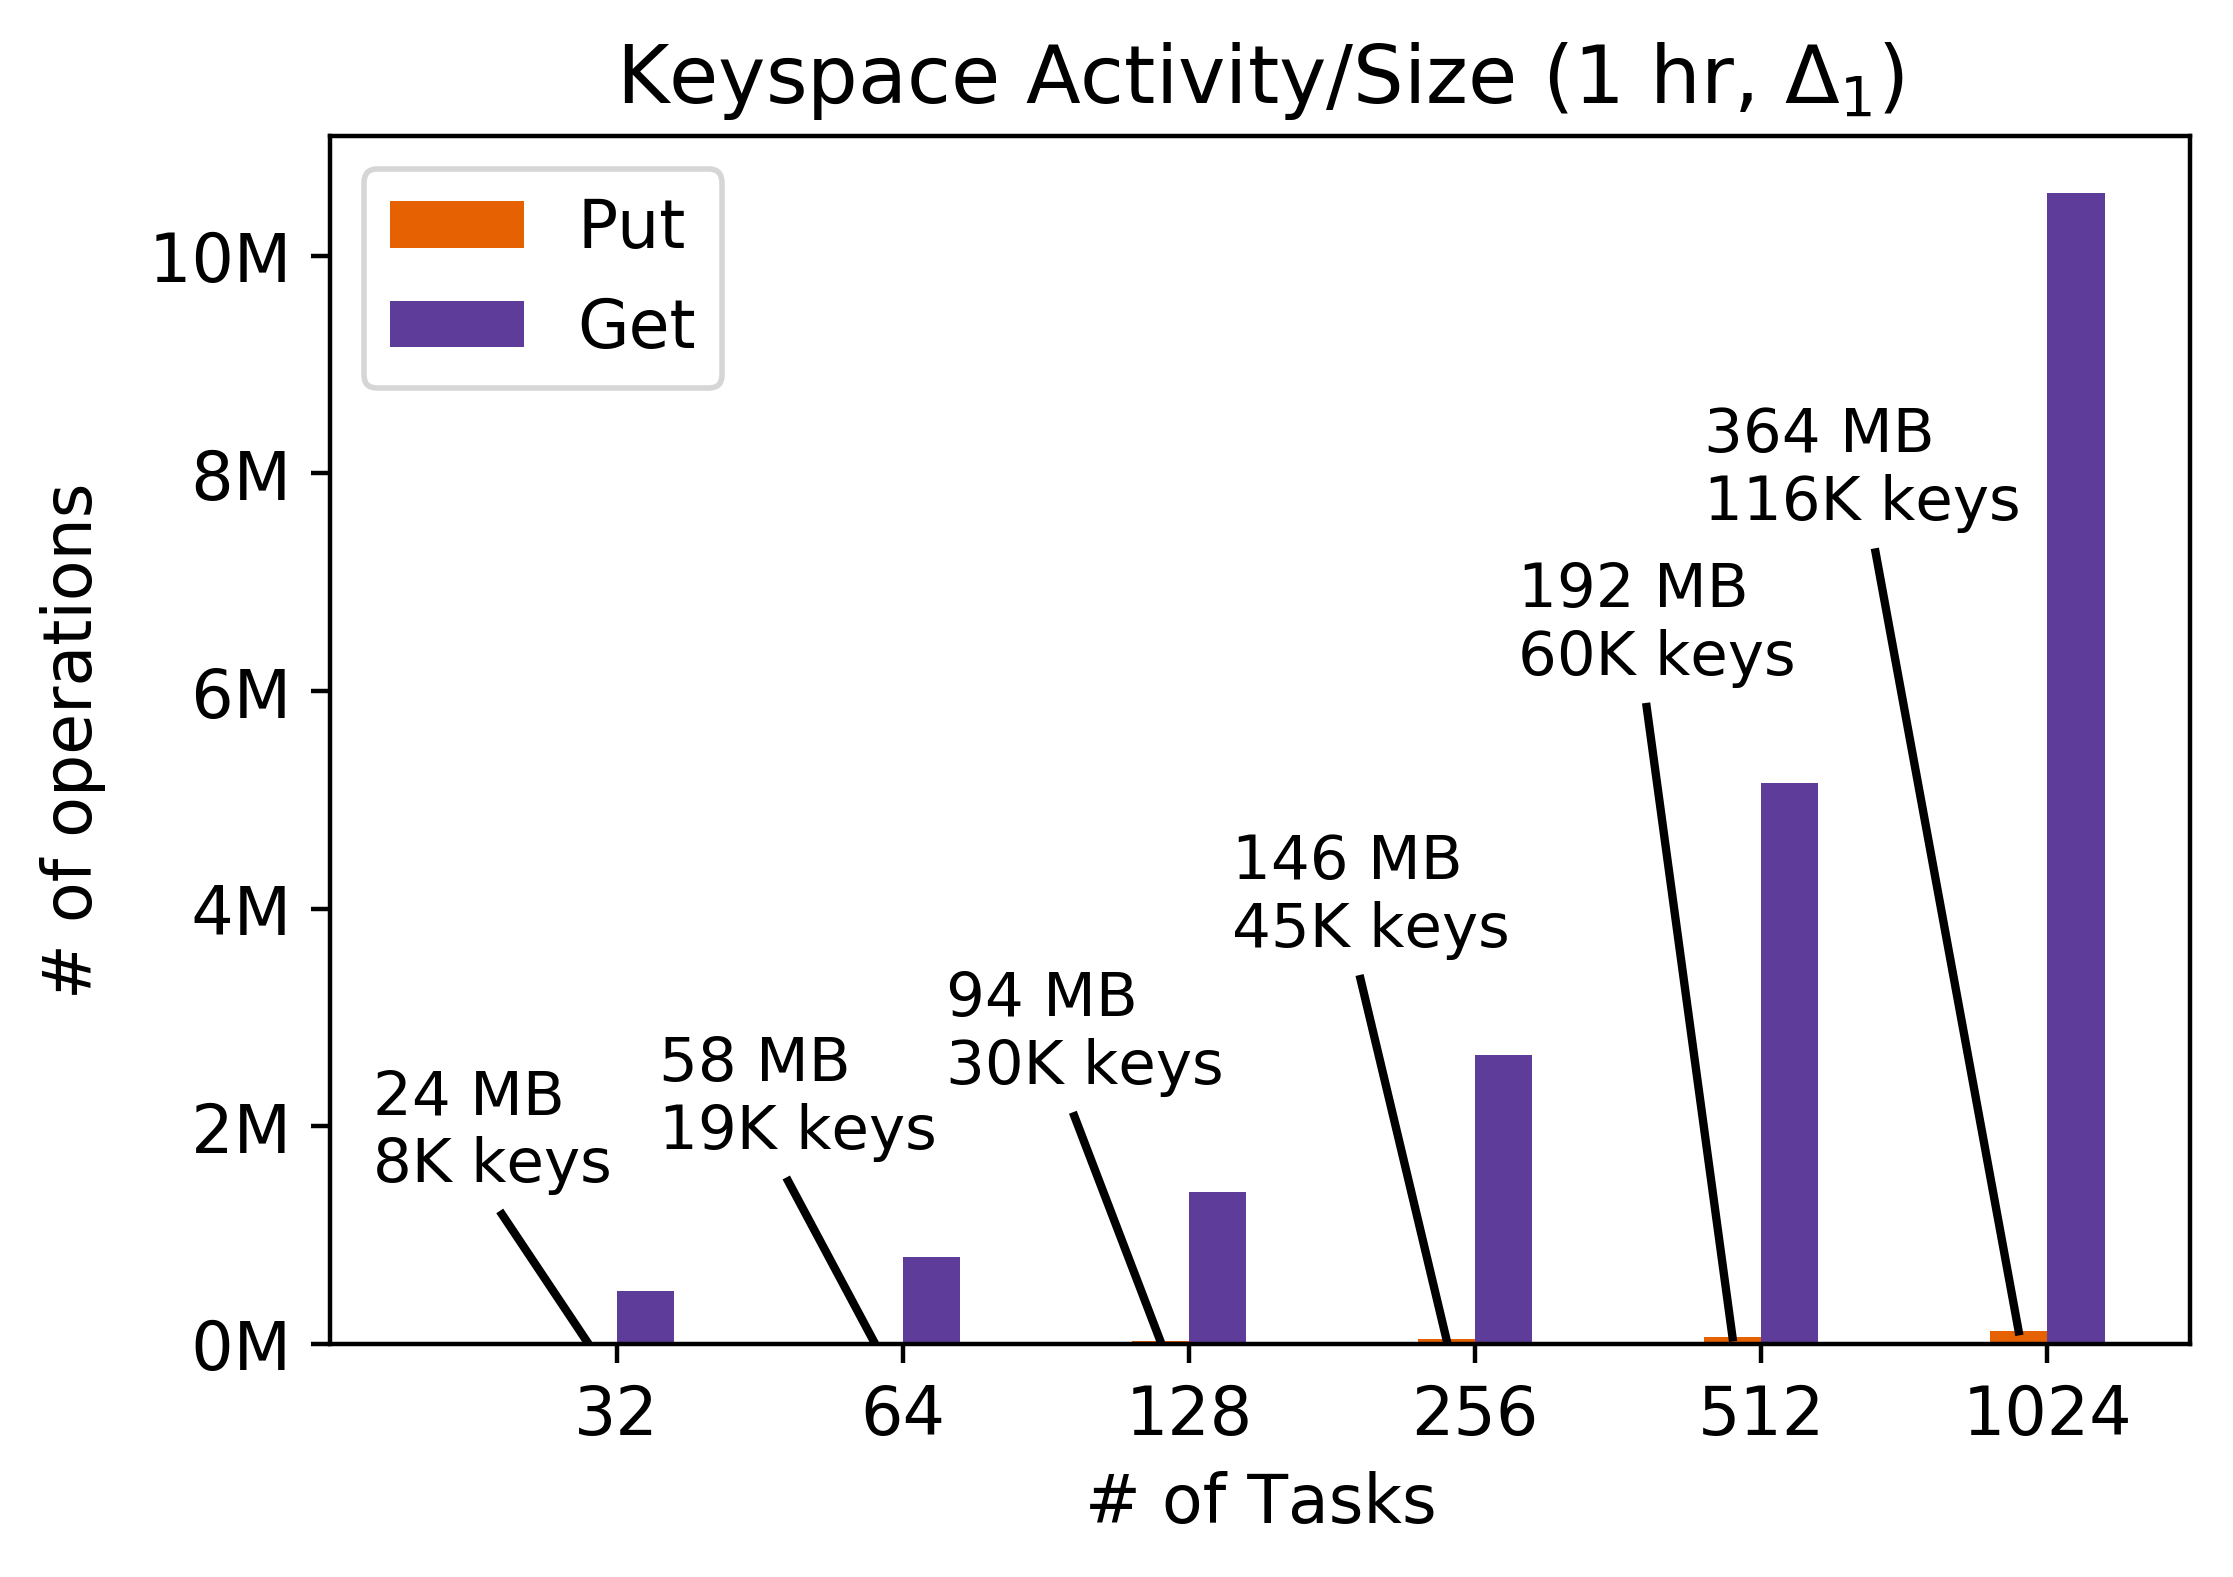
\includegraphics[width=0.5\textwidth]{figures/methodology-keyspace.png}\\
  \caption{The keyspace size is small but must satisfy many reads as workers
  calculate new segments. It is likely that we will need
  more than one node to manage segment coordinates when we scale the system or jobs up.
  \label{fig:methodology-keyspace}}
\end{figure}

\begin{figure}[t]
  \noindent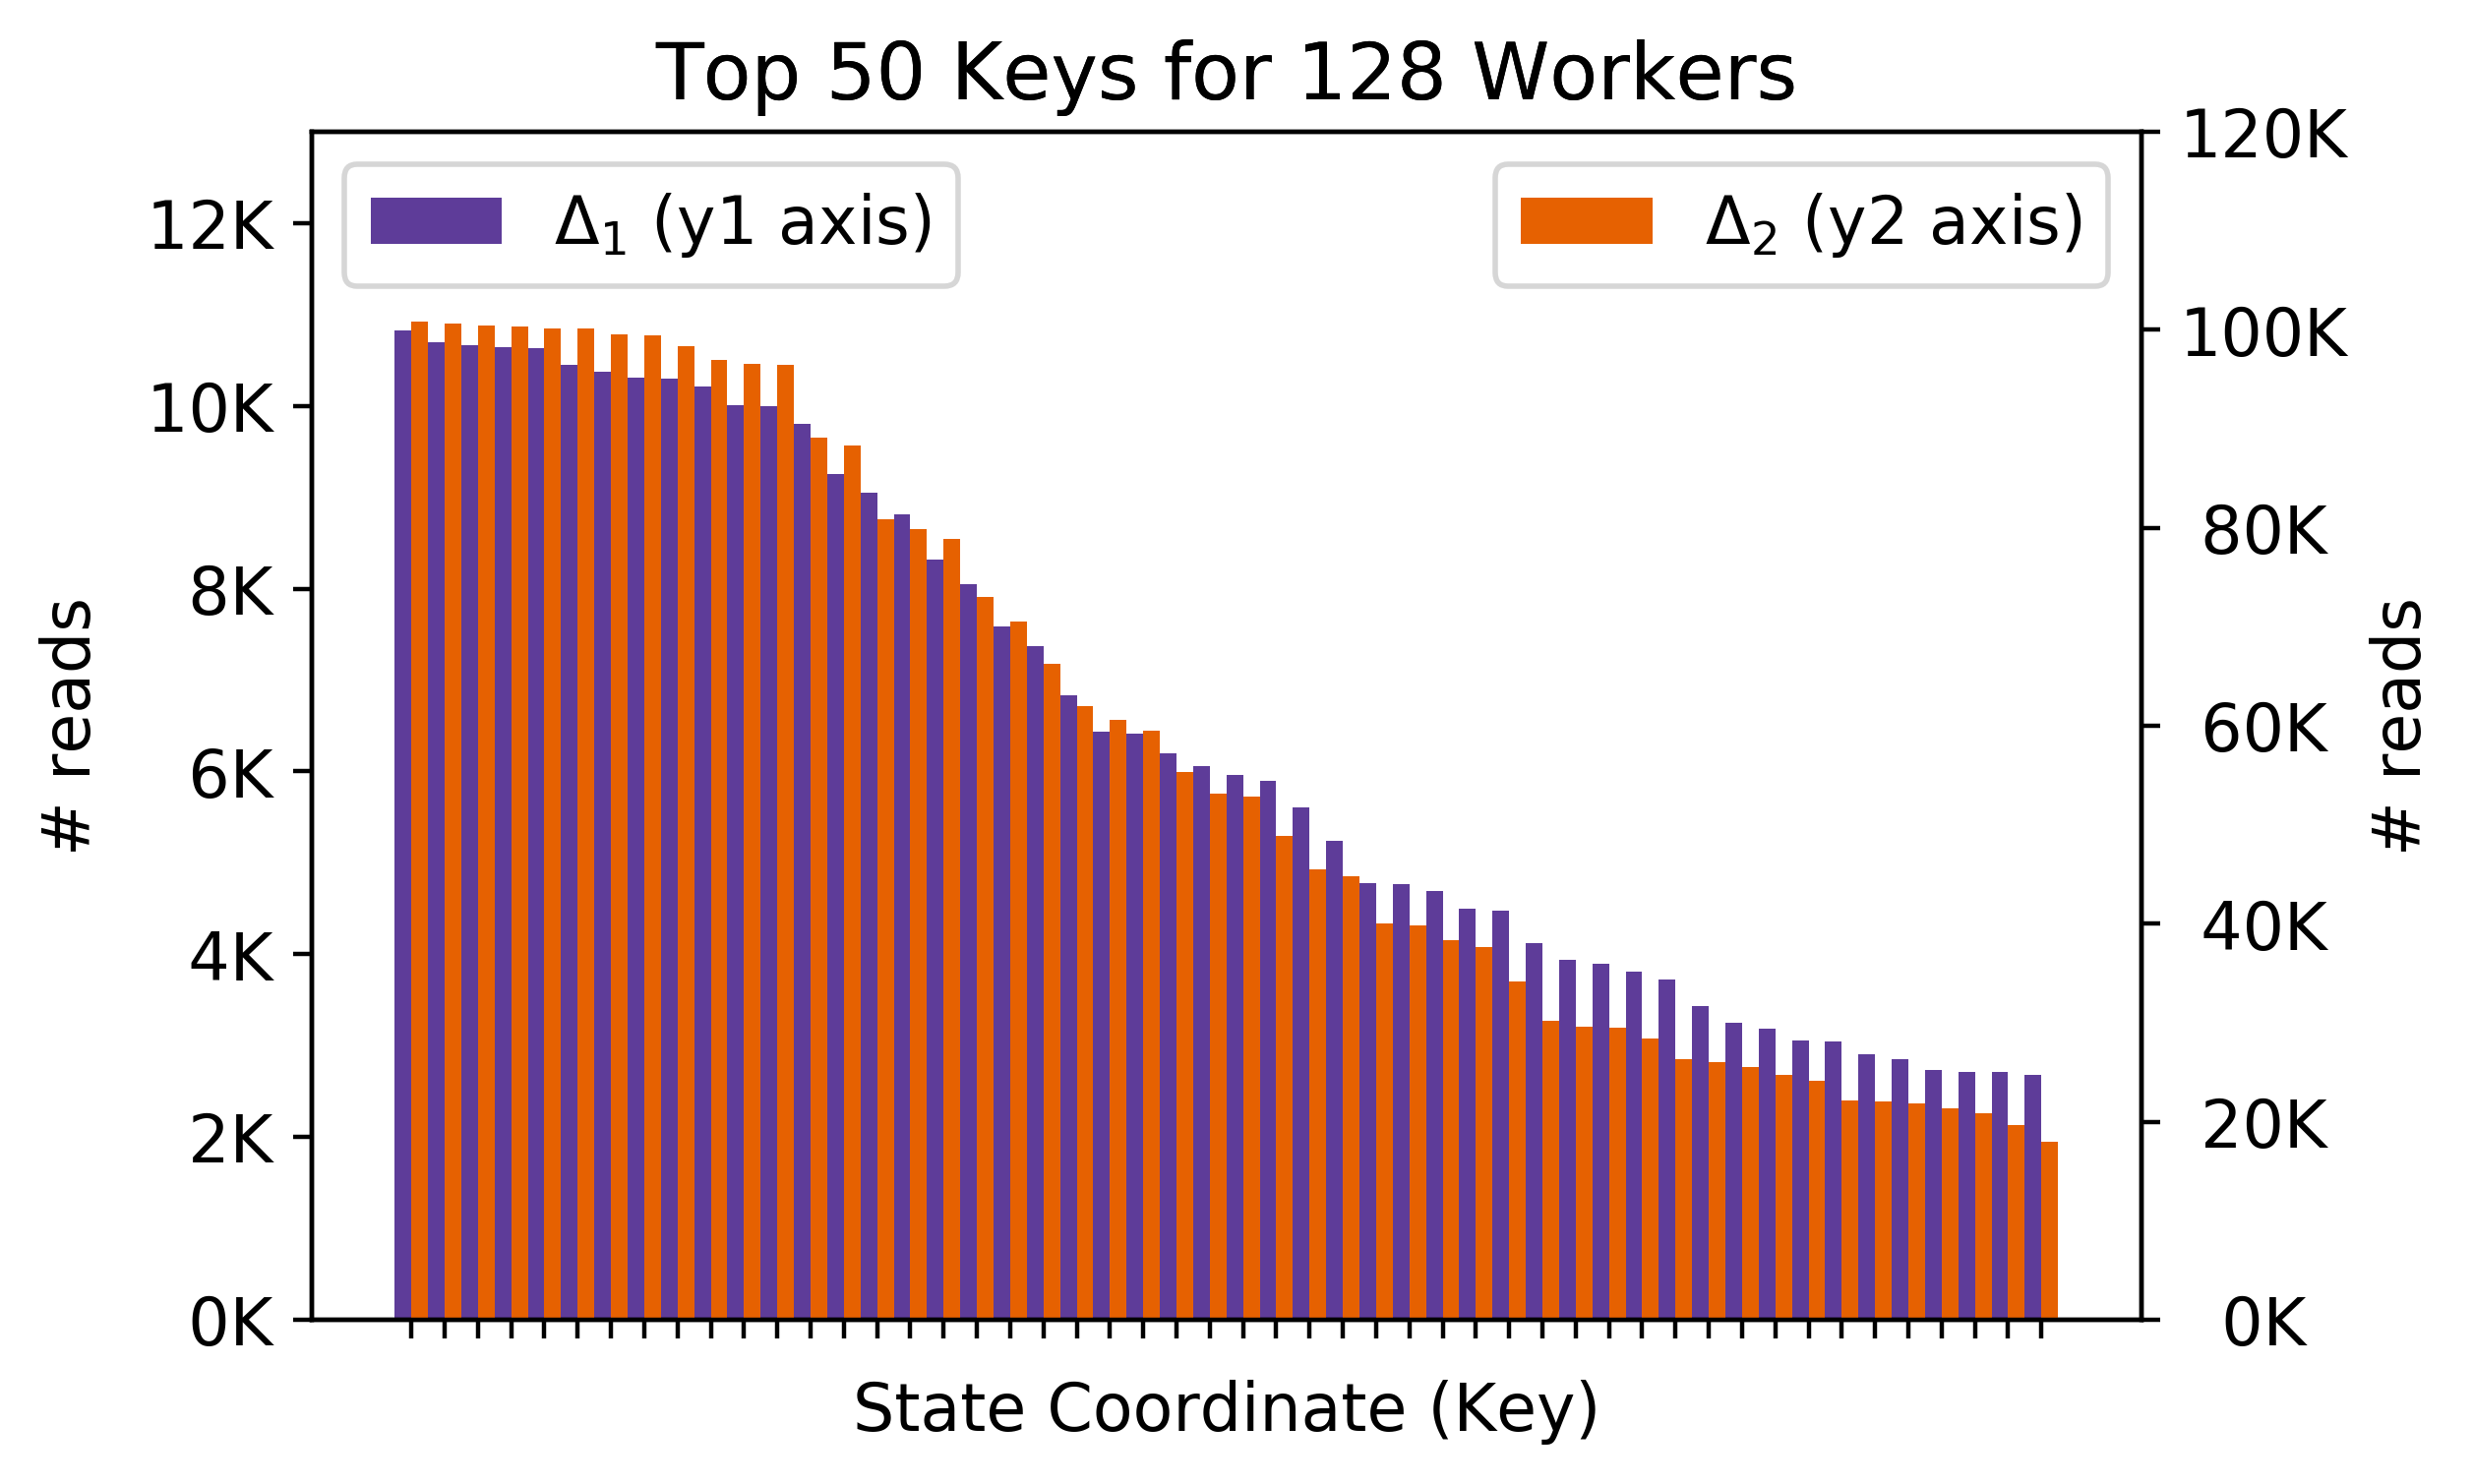
\includegraphics[width=0.5\textwidth]{figures/methodology-keys.png}\\
  \caption{The keyspace imbalance is due to workers generating deep
  trajectories and reading the same coordinates. Over time, the accesses get
  dispersed across different coordinates resulting in some keys being more
  popular than others.\label{fig:methodology-keys}}
\end{figure}

\subsubsection*{Scalability} Figure~\ref{fig:methodology-keyspace} shows the
keyspace size (text annotations) and request load (bars) after a one hour run
with a different number of workers (\(x\) axis). While the keyspace size and
capacity is relatively modest the memory usage scales linearly with the number
of workers. This is a problem if we want to scale to Trinitite's 6000 cores.
Furthermore, the size of the keyspace also increases linearly with the length
of the run.  Extrapolating these results puts an 8 hour run across all 100
Trinitite nodes at 20GB for the cache.  This memory utilization easily eclipses
the 3\% threshold we set earlier, even without factoring in the memory usage
from other workers.

\subsubsection*{An active but small keyspace} The bars in
Figure~\ref{fig:methodology-keyspace} show \(50-100\times\) as many reads
(\texttt{get()}) as writes (\texttt{put()}).  Worker tasks read the same key
for extended periods because the trajectory can remain stuck in so-called
superbasins composed of tightly connected sets of states. In this case, many
trajectory segments with the same coordinates are needed before the trajectory
moves on.  Writes only occur for the final state of segments generated by
worker tasks; their magnitude is smaller than reads because the caches ignore
redundant write requests. The number of read and write requests are highest at
the beginning of the run when worker tasks generate segments for the same
state, which is computationally cheap (this motivates
Section~\S\ref{sec:cache-management-using-system-archiecture-knowledge}).

\subsubsection*{Entropy increases over time} The reads per second in
Figure~\ref{fig:motivation-regimes} show that the number of requests decreases
and the number of active keys increases over time. The resulting key access
imbalance for the two growth rates in Figure~\ref{fig:motivation-regimes} are
shown in Figure~\ref{fig:methodology-keys}, where reads are plotted for each
unique state, or key, along the \(x\) axis. Keys are more popular than others
(up to \(5\times\)) because worker tasks start generating states with different
coordinates later in the run (this motivates
Section~\S\ref{sec:cache-management-using-domain-specific-knowledge}).  The
growth rate, temperature, and number of workers have a predictable effect on
the structure of the keyspace.  Figure~\ref{fig:methodology-keys} shows that
the number of reads changes with different initial conditions (\(\Delta\)), but
that the spatial locality of key accesses is similar ({\it e.g.}, some keys are
still \(5\times\) more popular than others).
Figure~\ref{fig:motivation-regimes} shows how entropy for different growth
rates has temporal locality, as the reads per second for \(\Delta_2\) looks
like the reads per second for \(\Delta_1\) stretched out along the time axis.
Trends also exist for temperature and number of workers but are omitted here
for space. This structure means that we can learn the regimes and adapt the
storage system (this motivates
Section~\S\ref{sec:cache-management-using-domain-specific-knowledge}).
